\documentclass[a4paper]{article}
\usepackage{header}

\usepackage{tikz}
\usepackage{tikz-network}
\usepackage{float}

\newcommand\enumtocitem[3]{\item\textbf{#1}\addtocounter{#2}{1}\addcontentsline{toc}{#2}{\protect{\numberline{#3}} #1}}
\newcommand\defitem[1]{\enumtocitem{#1}{subsection}{\thesubsection}}
\newcommand\proofitem[1]{\enumtocitem{#1}{subsection}{\thesubsection}}

\newlist{colloq}{enumerate}{1}
\setlist[colloq]{leftmargin=*,label=\textbf{\arabic*.}}

\graphicspath{
    {img/}
}


\title{\HugeДискретная математика, Коллоквиум 2}
\author{
	Балюк Игорь \\
	\href{https://teleg.run/lodthe}{@lodthe},
    \href{https://github.com/LoDThe/hse-tex}{GitHub} \\
}
\date{2019 --- 2020}

\begin{document}
    \maketitle

    Материалы взяты из учебника Александра Рубцова.

    \tableofcontents

    \newpage

    \section{Определения}

    Контрольный вопрос на понимание определений включает в себя формулировку одного определения из списка ниже и контрольный вопрос по этому определению. Пример: <<Определение полного прообраза. Пусть $f(x) = x^2$ --- функция из $\ZZ$ в $\ZZ$. Найдите полный прообраз множества $\{1, 2, 3, 4\}$.

    \begin{colloq}
    
    \defitem{Деление целых чисел с остатком.}

        Говорят, что целое число $a$ делится на целое число $b$, если $a = bk$ для некоторого целого числа $k$. В этом случае говорят также <<$a$ кратно $b$>>, и <<$b$ является делителем числа $a$>>.

        Теперь определим деление $с$ остатком. Пусть $b$ --- целое положительное число. Деля на $b$ с остатком, мы связываем  предметы в пачки по $b$ в каждой, пока это возможно: количество полных пачек называется частным (говорят ещё <<неполное частное>>, чтобы отличать от частного как дроби), и сколько-то предметов останется, их количество и называют остатком.

        Формально: разделить целое $a$ на целое положительное $b$ означает найти такое целое $q$ (\textit{частное}) и такое $r$ (\textit{остаток}), что
        \begin{equation*}
            a = b \cdot q + r; \quad 0 \leq r < b.
        \end{equation*}


    \defitem{Сравнения по модулю. Основные свойства.}

        Если два числа $a$ и $b$ дают одинаковые остатки при делении на положительное число $N$, то говорят, что они \textit{сравнимы} по модулю $N$, и пишут $a \equiv b \pmod N$.

        Эквивалентное определение: $a$ и $b$ сравнимы по модулю $N$, если разность $a - b$ делится на $N$. В самом деле, если они дают одинаковый остаток $r$, то $a = k \cdot N + r$, $b = l \cdot N + r$, и $a - b = k \cdot N - l \cdot N = (k - l) \cdot N$ . Наоборот, если $a - b = m \cdot N$, и $b$ даёт остаток $r$, то $b = l \cdot N + r$ и $a = (a - b) + b = m \cdot N + l \cdot N + r = (m + l) \cdot N + r$, то есть $a$ даёт тот же остаток $r$.

        Можно сказать, что при данном $N$ все целые числа разбиваются на $N$ классов в зависимости от остатков по модулю $N$: два числа в одном классе сравнимы, а числа в разных классах --- нет.

        Важное свойство сравнений: чтобы узнать, в какой класс попадет сумма или произведение двух чисел, достаточно знать, в каком классе лежат слагаемые или сомножители: если одно из слагаемых (один из сомножителей) изменить на кратное $N$, то сумма (произведение) тоже изменится на кратное $N$.
            
        В самом деле, если к одному из слагаемых прибавить $k \cdot N$, то к сумме тоже прибавится $k \cdot N$, аналогично для разности. С произведением: $(a + k \cdot N) \cdot b = a \cdot b + k \cdot b \cdot N \equiv a \cdot b \pmod N$.

        Благодаря этому свойству в выражении, содержащем операции сложения и умножения (или возведение в целую степень, которое сводится к многократному умножению), можно заменять слагаемые или сомножители на сравнимые по модулю $N$ --- если результат нам важен лишь по модулю $N$.
        
        Например, можно найти $2^{100} \bmod 7$ (остаток от деления $2^{100}$ на $7$): поскольку $2^3 = 8 \equiv 1 \pmod 7$, то $2^{99} = (2^{3})^{33} \equiv 1^{33} = 1 \pmod 7$, так что $2^{100} = 2^{99} \cdot 2 \equiv 1 \cdot 2 = 2 \pmod 7$.

    \defitem{Арифметика остатков (вычетов). Обратимые остатки (вычеты).}

        Остаток (вычет) по модулю $N$ называется \textbf{обратимым}, если в произведении с каким-то другим остатком он даёт $1$. Другими словами, $a$ обратим, если уравнение $a \cdot x \equiv 1 \pmod N$ имеет решение.

    \defitem{Малая теорема Ферма.}

        \begin{theorem*}
            Если $p$ --- простое число, то
            \begin{equation*}
                a^{p - 1} \equiv 1 \pmod p
            \end{equation*}
            при любом $a$, не делящемся на $p$.
        \end{theorem*}

    \defitem{Функция Эйлера. Теорема Эйлера.}

        \begin{theorem*}
            Пусть $N > 1$ --- произвольное целое число, а $\phi(N)$ равно количеству остатков среди $0, 1, \dots, N - 1$, взаимно простых с $N$. Пусть $a$ --- один из этих остатков. Тогда
            \begin{equation*}
                a^{\phi(N)} \equiv 1 \pmod N.
            \end{equation*}
        \end{theorem*}

        Функцию $\phi$ называют \textbf{функцией Эйлера} и традиционно обозначают буквой $\phi$.  Если $N$ простое, то $\phi(N) = N - 1$, и теорема Эйлера превращается в малую теорему Ферма.

    \defitem{Наибольший общий делитель. Алгоритм Евклида.}

        Наибольшим общим делителем (НОД) для двух целых чисел $m$ и $n$ называется наибольший из их общих делителей. Пример: для чисел $54$ и $24$ наибольший общий делитель равен $6$.

        Алгоритм нахождения НОДа алгоритмом Евклида:
        \begin{enumerate}
            \item
                Большее число делим на меньшее.
            \item
                Если делится без остатка, то меньшее число и есть НОД (следует выйти из цикла).
            \item
                Если есть остаток, то большее число заменяем на остаток от деления.
            \item
                Переходим к пункту 1.
        \end{enumerate}

    \defitem{Расширенный алгоритм Евклида нахождения решения линейного диофантова уравнения.}

    \defitem{Простые числа, формулировка основной теоремы арифметики.}
 
        Целое число $p > 1$ называется простым, если оно не разлагается в произведение меньших чисел (то есть не имеет положительных делителей, кроме $1$ и $p$).

        \begin{theorem*}
            Всякое целое положительное число, большее $1$, разлагается на простые множители, причём единственным образом: любые два разложения отличаются только перестановкой сомножителей.
        \end{theorem*}

    \defitem{Равномощные множества.}

        Множество $A$ называется равномощным множеству $B$, если существует биекция множества $A$ в множество $B$.

    \defitem{Cчётные множества.}

        Множество называется счётным, если оно равномощно множеству натуральных чисел $\NN$.

    \defitem{Множества мощности континуум.}

        Множество имеет мощность \textbf{континуум}, если оно равномощно $\RR$.

    \defitem{Основные определения элементарной теории вероятностей: исходы, события, вероятность события.}

        \textbf{Вероятностным пространством} называется конечное множество $U$, его элементы называются \textbf{возможными исходами}. \textbf{Событием} называется произвольное подмножество $A \subseteq U$. 

        На вероятностном пространстве задана функция $Pr: U \to [0; 1]$, такая что $\sum_{x \in U} Pr[x] = 1$. Функция $Pr$ называется \textbf{вероятностным распределением}, а число $Pr[x]$ называется \textbf{вероятностью исхода} $x \in U$. Вероятностью события $A$ называется число $Pr[A] = \sum_{x \in A} Pr[x]$.

    \defitem{Формулировка формулы включений и исключений для вероятностей.}

        В равновозможной модели для произвольных множеств $A_1, \dots, A_n \subseteq U$ верно
        \begin{equation*}
            Pr[A_1 \cup A_2 \cup \dots \cup A_n] = \sum_i Pr[A_i] - \sum_{i < j} Pr[A_i \cap A_j] + \dots = \sum_{\varnothing \neq I \subseteq \{1, 2, \dots, n\}} (-1)^{|I| + 1} Pr\left[\bigcap_{i \in I} A_i\right].
        \end{equation*}

    \defitem{Условная вероятность.}

        Помимо вероятностей тех или иных событий бывает нужным говорить и о вероятностях одних событий при условии других. Неформально говоря, мы хотим определить вероятность выполнения события $A$ в том случае, когда событие $B$ выполняется. 
        
        В терминах вероятностного пространства определение этого понятия довольно естественное: нужно сузить вероятностное пространство на множество $B$. Так, для равновозможной модели мы получаем, что вероятность $A$ при условии $B$ есть просто $\dfrac{|A \cap B|}{|B|}$, то есть число благоприятных исходов поделенное на число всех исходов (после сужения всего вероятностного пространства до $B$). 
        
        В случае произвольного вероятностного пространства нужно учесть веса исходов, то есть нужно сложить вероятности исходов в $A \cap B$ и поделить на сумму вероятностей исходов в $B$.

        Таким образом, мы приходим к формальному определению. \textbf{Условной вероятностью} события $A$ при условии $B$ называется число
        \begin{equation*}
            Pr[A \mid B] = \dfrac{Pr[A \cap B]}{\Pr[B]}.
        \end{equation*}


    \defitem{Независимые события. Основные свойства независимых событий.}

        События $A$ и $B$ называются независимыми, если
        \begin{equation*}
            Pr[A] = Pr[A \mid B].
        \end{equation*}

        Из определения условной вероятности мы сразу получаем эквивалентное определение независимостей событий. Событие $A$ не зависит от события $B$, если
        \begin{equation*}
            Pr[A \cap B] = Pr[A] \cdot Pr[B].
        \end{equation*}

    \defitem{Формула полной вероятности.}

        \begin{lemma*}
            Пусть $B_1, B_2, \dots, B_n$ --- разбиение вероятностного пространства, то есть $U = B_1 \cup B_2 \cup \dots \cup B_n$, где $B_i \cap B_j = \varnothing$ при $i \neq j$. Пусть также $Pr[B_i] > 0$ для всякого $i$. Тогда для всякого события $A$
            \begin{equation*}
                Pr[A] = \sum_{i = 1}^n Pr[A \mid B_i] \cdot Pr[B_i].
            \end{equation*}
        \end{lemma*}

    \defitem{Случайная величина и математическое ожидание. Линейность математического ожидания.}

        \textbf{Случайная величина} --- это числовая функция на вероятностном пространстве, то есть функция вида $\xi: U \to \RR$. То есть, по сути, случайная величина --- это обычная числовая функция, но теперь на её аргументах задано вероятностное распределение.

        \textbf{Математическим ожиданием} случайной величины $\xi: U \to \RR$ называется число
        \begin{equation*}
            E[\xi] = \sum_{u \in U} \xi(u) \cdot Pr[u]
        \end{equation*}

        \begin{lemma*} (линейность математического ожидания) 
            Пусть $\xi: U \to \RR$ и $g: U \to \RR$ --- две случайные величины на одном и том же вероятностном пространстве. Тогда
            \begin{equation*}
                E[f + g] = E[f] + E[g].
            \end{equation*}
        \end{lemma*}

    \defitem{Формулировка неравенства Маркова.}

        \begin{lemma*}
            Пусть $\xi$ --- случайная величина, принимающая только \textbf{неотрицательные} значения. Тогда для всякого $x > 0$ верно
            \begin{equation*}
                Pr[\xi \geq x] \leq \dfrac{E[\xi]}{x}.
            \end{equation*}
        \end{lemma*}

        То есть, вероятность того, что случайная величина $\xi$ сильно больше своего математического ожидания, не слишком велика (заметим, что лемма становится содержательной, когда $x > E[\xi]$).

    \defitem{Определение схемы в некотором функциональном базисе. Представление схем графами.}

        \textbf{Полным базисом} называется набор связок, если через эти связки выражается любая булева функция.

        \textbf{Стандартным базисом} назовём набор из операций конъюнкция (И), дизъюнкция (ИЛИ) и отрицание (НЕ). 

        \textbf{Булевой схемой} от переменных $x_1, \dots, x_n$ мы будем называть последовательность булевых функций $g_1, \dots, g_s$, в которой всякая $g_i$ получается из предыдущих функций последовательности и переменных применением одной из логических операций из выбранного базиса для этой схемы.

        В булевой схеме задано некое число $m \geq 1$ и члены последовательности $g_{s - m + 1}, \dots, g_s$ называются \textbf{выходами схемы}. Число $m$ называют числом выходов схемы.

        Мы говорим, что схема вычисляет булеву функцию $f: \{0, 1\}^n \to \{0, 1\}^m$, если для всякого $x \in \{0, 1\}^n$ верно $f(x) = (g_{s - m + 1}(x), \dots, g_{s}(x))$.

        \textbf{Размером} схемы называют число $s$.

        Рассмотрим представление схемы графом:
        \begin{figure}[H]
            \caption{Схема функции $x_1 \oplus x_2$}
            \centering
            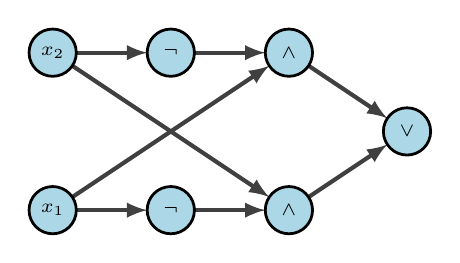
\begin{tikzpicture}
                \Vertex[y=0,x=0,label=$x_1$]{x1}
                \Vertex[y=2,x=0,label=$x_2$]{x2}
                \Vertex[y=0,x=1.5,label=$\neg$]{nx1}
                \Vertex[y=2,x=1.5,label=$\neg$]{nx2}
                \Vertex[y=0,x=3,label=$\land$]{ax1}
                \Vertex[y=2,x=3,label=$\land$]{ax2}
                \Vertex[y=1,x=4.5,label=$\lor$]{end}
                \Edge[Direct](x1)(nx1)
                \Edge[Direct](x2)(nx2)
                \Edge[Direct](nx1)(ax1)
                \Edge[Direct](x2)(ax1)
                \Edge[Direct](nx2)(ax2)
                \Edge[Direct](x1)(ax2)
                \Edge[Direct](ax1)(end)
                \Edge[Direct](ax2)(end)
            \end{tikzpicture}
        \end{figure}

    \defitem{Полный базис. Примеры полных и неполных базисов.}

    \defitem{Полином Жегалкина (в стандартном виде).}

        \textbf{Многочленом Жегалкина} называется формула вида
        \begin{equation*}
            \bigoplus_{S \subseteq \{1, \dots, n\}} a_S \bigwedge_{i \in S} x_i, \quad a_S \in \{0, 1\}.
        \end{equation*}

        Примеры многочлена Жегалкина:
        \[\begin{gathered}
            1 \oplus x_1 \oplus x_2 \oplus x_3 \oplus (x_1 \land x_2) \oplus (x_1 \land x_3) \oplus (x_2 \land x_3) \oplus (x_1 \land x_2 \land x_3); \\
            x_3 \oplus (x_1 \land x_3) \oplus (x_2 \land x_3) \oplus (x_1 \land x_2 \land x_3).
        \end{gathered}\]

        Для простоты чтения $\land$ можно опускать:
        \begin{equation*}
            1 \oplus x_1 \oplus x_2 \oplus x_3 \oplus x_1 x_2 \oplus x_1 x_3 \oplus x_2 x_3 \oplus x_1 x_2 x_3; \\
        \end{equation*}

    \defitem{Схемная сложность функции (размер схемы).}

        \textbf{Схемная сложность} булева отображения $f: \{0, 1\}^n \to \{0, 1\}^m$ (в частности, булевой функции) --- это наименьший размер схемы, вычисляющей это выражение.

    \end{colloq}

    \section{Вопросы на знание доказательств}
    \begin{colloq}
    \setlength\parindent{20pt}

    \proofitem{Сравнение $ax \equiv 1 \pmod{N}$ имеет решение тогда и только тогда, когда $\text{НОД}(a, N) = 1$.}
    \proofitem{Малая теорема Ферма.}
    \proofitem{Теорема Эйлера.}
    \proofitem{Корректность алгоритма Евклида и расширенного алгоритма Евклида.}
    \proofitem{Основная теорема арифметики.}
    \proofitem{Китайская теорема об остатках.}
    \proofitem{Мультипликативность функции Эйлера. Формула для функции Эйлера.}
    \proofitem{Формула Байеса. Формула полной вероятности.}
    \proofitem{Парадокс дней рождений (математическое ожидание числа людей с совпавшими днями рождений)}
    \proofitem{Неравенство Маркова.}
    \proofitem{Нижняя оценка на максимальное количество ребер в разрезе.}
    \proofitem{Любое бесконечное множество содержит счётное подмножество. Любое подмножество счётного множества конечно или счётно.}
    \proofitem{Конечное или счётное объединение конечных или счётных множеств конечно или счётно}
    \proofitem{Счётность декартова произведения счетных множеств. Счётность множества рациональных чисел.}
    \proofitem{Равномощность отрезков, интервалов, лучей и прямых (явные биекции).}
    \proofitem{Несчетность множества бесконечных двоичных последовательностей.}
    \proofitem{Теорема Кантора-Бернштейна.}
    \proofitem{Нижняя оценка на число монотонных булевых функций: монотонных булевых функций от $2n$ переменных не меньше $2^{\frac{2^n}{2n + 1}}$}
    \proofitem{Существование и единственность полинома Жегалкина (в стандартном виде) для любой булевой функции.}
    \proofitem{Разложение в ДНФ и КНФ булевой функции.}
    \proofitem{Верхняя оценка $O(n 2^n)$ схемной сложности булевой функции от $n$ переменных.}
    \proofitem{Булевы схемы для сложения и умножения n-битовых чисел. Оценка размера.}
    \proofitem{Булева схема для задачи о связности графа. Оценка размера.}
    \proofitem{Задача об угадывании числа. Верхняя и нижняя оценки.}
    \proofitem{Задача о сортировке нижняя оценка.}
    \proofitem{Задача о нахождении самой тяжелой монеты. Верхние и нижние оценки.}

    \end{colloq}

\end{document}